% %%%%%%%%%%%%%%%%%%%%%%%%%%%%%%%%%%%%%%%%%%%%%%%%%%%%%%%%%%%%%%%%%%%%%%%%%%%%%%%%
\documentclass{article}
\usepackage[a4paper, hmargin={2.8cm, 2.8cm}, vmargin={2.5cm, 2.5cm}]{geometry}
% %%%%%%%%%%%%%%%%%%%%%%%%%%%%%%%%%%%%%%%%%%%%%%%%%%%%%%%%%%%%%%%%%%%%%%%%%%%%%%%%

% %%%%%%%%%%%%%%%%%%%%%%%%%%%%%%%%%%%%%%%%%%%%%%%%%%%%%%%%%%%%%%%%%%%%%%%%%%%%%%%%
\usepackage[utf8]{inputenc}
\usepackage[T1]{fontenc}
% %%%%%%%%%%%%%%%%%%%%%%%%%%%%%%%%%%%%%%%%%%%%%%%%%%%%%%%%%%%%%%%%%%%%%%%%%%%%%%%%


% %%%%%%%%%%%%%%%%%%%%%%%%%%%%%%%%%%%%%%%%%%%%%%%%%%%%%%%%%%%%%%%%%%%%%%%%%%%%%%%%
\usepackage{mathtools}
\usepackage{amsthm}
\usepackage{amssymb}
\usepackage{csvsimple}
\usepackage{subcaption}
\usepackage{url}
\usepackage{tikz}\usepackage{pgfplots}

% %%%%%%%%%%%%%%%%%%%%%%%%%%%%%%%%%%%%%%%%%%%%%%%%%%%%%%%%%%%%%%%%%%%%%%%%%%%%%%%%


% %%%%%%%%%%%%%%%%%%%%%%%%%%%%%%%%%%%%%%%%%%%%%%%%%%%%%%%%%%%%%%%%%%%%%%%%%%%%%%%%
\usepackage{fancyhdr}
\usepackage{graphicx}
\usepackage{parskip}
\usepackage{listings}
\usepackage{enumitem}
\usepackage{titlesec}
\usepackage[lastpage,user]{zref}
\usepackage{caption}
\usepackage{scrextend}
\usepackage[outputdir=./.latex-out]{minted} % TODO remove if you don't use minted
\usepackage{listings}
\usepackage{blindtext}
% %%%%%%%%%%%%%%%%%%%%%%%%%%%%%%%%%%%%%%%%%%%%%%%%%%%%%%%%%%%%%%%%%%%%%%%%%%%%%%%%
\newcommand{\python}[1] {
  \mintinline{python}{#1}
}
\newcommand{\tex}[1] {
  \mintinline{latex}{#1}
}
\pagestyle{fancy}
% %%%%%%%%%%%%%%%%%%%%%%%%%%%%%%%%%%%%%%%%%%%%%%%%%%%%%%%%%%%%%%%%%%%%%%%%%%%%%%%%
% %%%%%%%%%%%%%%%%%%%%%%%%%%%%%%%%%%%%%%%%%%%%%%%%%%%%%%%%%%%%%%%%%%%%%%%%%%%%%%%%
\lhead{\LaTeX webinar} % TODO insert left page header
\rhead{Study Now} % TODO insert right page header
\cfoot{\thepage\ of \zpageref{LastPage}}
\newtheorem*{prp}{Propostion}
\setlist{nolistsep}
% %%%%%%%%%%%%%%%%%%%%%%%%%%%%%%%%%%%%%%%%%%%%%%%%%%%%%%%%%%%%%%%%%%%%%%%%%%%%

% %%%%%%%%%%%%%%%%%%%%%%%%%%%%%%%%%%%%%%%%%%%%%%%%%%%%%%%%%%%%%%%%%%%%%%%%%%%%
\title{
  \vspace{13em}
  \large{Study Now} \\
  \Large{\LaTeX{} webinar} \\
}

\author{
  Benjamin Rotendahl --- Benjamin@Rotendahl.dk
}

\date{
  \vspace{22em}
  \today
}
% %%%%%%%%%%%%%%%%%%%%%%%%%%%%%%%%%%%%%%%%%%%%%%%%%%%%%%%%%%%%%%%%%%%%%%%%%%%%
% %%%%%%%%%%%%%%%%%%%%%%%%%%%%%%%%%%%%%%%%%%%%%%%%%%%%%%%%%%%%%%%%%%%%%%%%%%%%%%%%

\begin{document}

\clearpage

% % The following lines creates the title, table of contents and the frontpage
% %%%%%%%%%%%%%%%%%%%%%%%%%%%%%%%%%%%%%%%%%%%%%%%%%%%%%%%%%%%%%%%%%%%%%%%%%%%%%
\maketitle
\thispagestyle{empty}
\newpage

\thispagestyle{empty}\tableofcontents\newpage % TODO remove this line to remove table of contents

\setcounter{page}{1}
%%%%%%%%%%%%%%%%%%%%%%%%%%%%%%%%%%%%%%%%%%%%%%%%%%%%%%%%%%%%%%%%%%%%%%%%%%%%%

\section{Introduction}
This document is as a \emph{cheat sheet}. It covers how to setup a \LaTeX{}
document and showcases the most common \LaTeX{} commands and functions. You
have both the pdf and source code such that you can add other cool commands
you find on your journey.

\section{\LaTeX{} background}
Before diving into the syntax of \LaTeX{} you should know a bit about the
process of writing \LaTeX{} documents. \LaTeX{} is a typesetting program and
language. The main advantage of \LaTeX{} is its ability to typeset math, code
and other scientific/technical figures. \LaTeX{} in an extension of TeX, which
released by Donald Knuth in the year 1981.

\subsection{From source code to PDF}\label{sec:local}
\LaTeX{} is not a word processor, but a language and compiler which given a
file containing source code, written in an \emph{editor}, creates a PDF.
as mentiond in section~\ref{sec:local}


An editor for local use, could be \emph{Visual studio code}\cite{vscode}, it
can be used to write any programming/markup language. Support for languages
comes through packages that extends its functionality, there exists packages
for most languages such as python, javascript and \LaTeX{}\cite{latexPackage}.

After the editor has saved the source code, it must be passed to the compiler.
This can be setup to happen automatically on save. There are different versions
of the compiler, they differ in the amount of packages and features they come
with.  ``The latex project TeX''\cite{texLive} has links to various distributions
for the most common operating systems.
With an editor and compiler installed you are ready to write \LaTeX{}.
The processes is illustrated in figure~\ref{fig:compile}.


\subsubsection{Overleaf}
Section~\ref{sec:local} explains how to create a \LaTeX{} setup on your own
computer. There exists services such as Overleaf\footnote{\url{overleaf.com}},
they are to \LaTeX{} what Google docs is to Microsoft Word. They live in the
browser and give you a full environment, no installation required. This makes
it easier to share documents with potential group members, but has the
disadvantage that they require an internet connection to function.They are
also more limited in the amount of configuration options and packages available.

\begin{figure}[h]
	\centering
	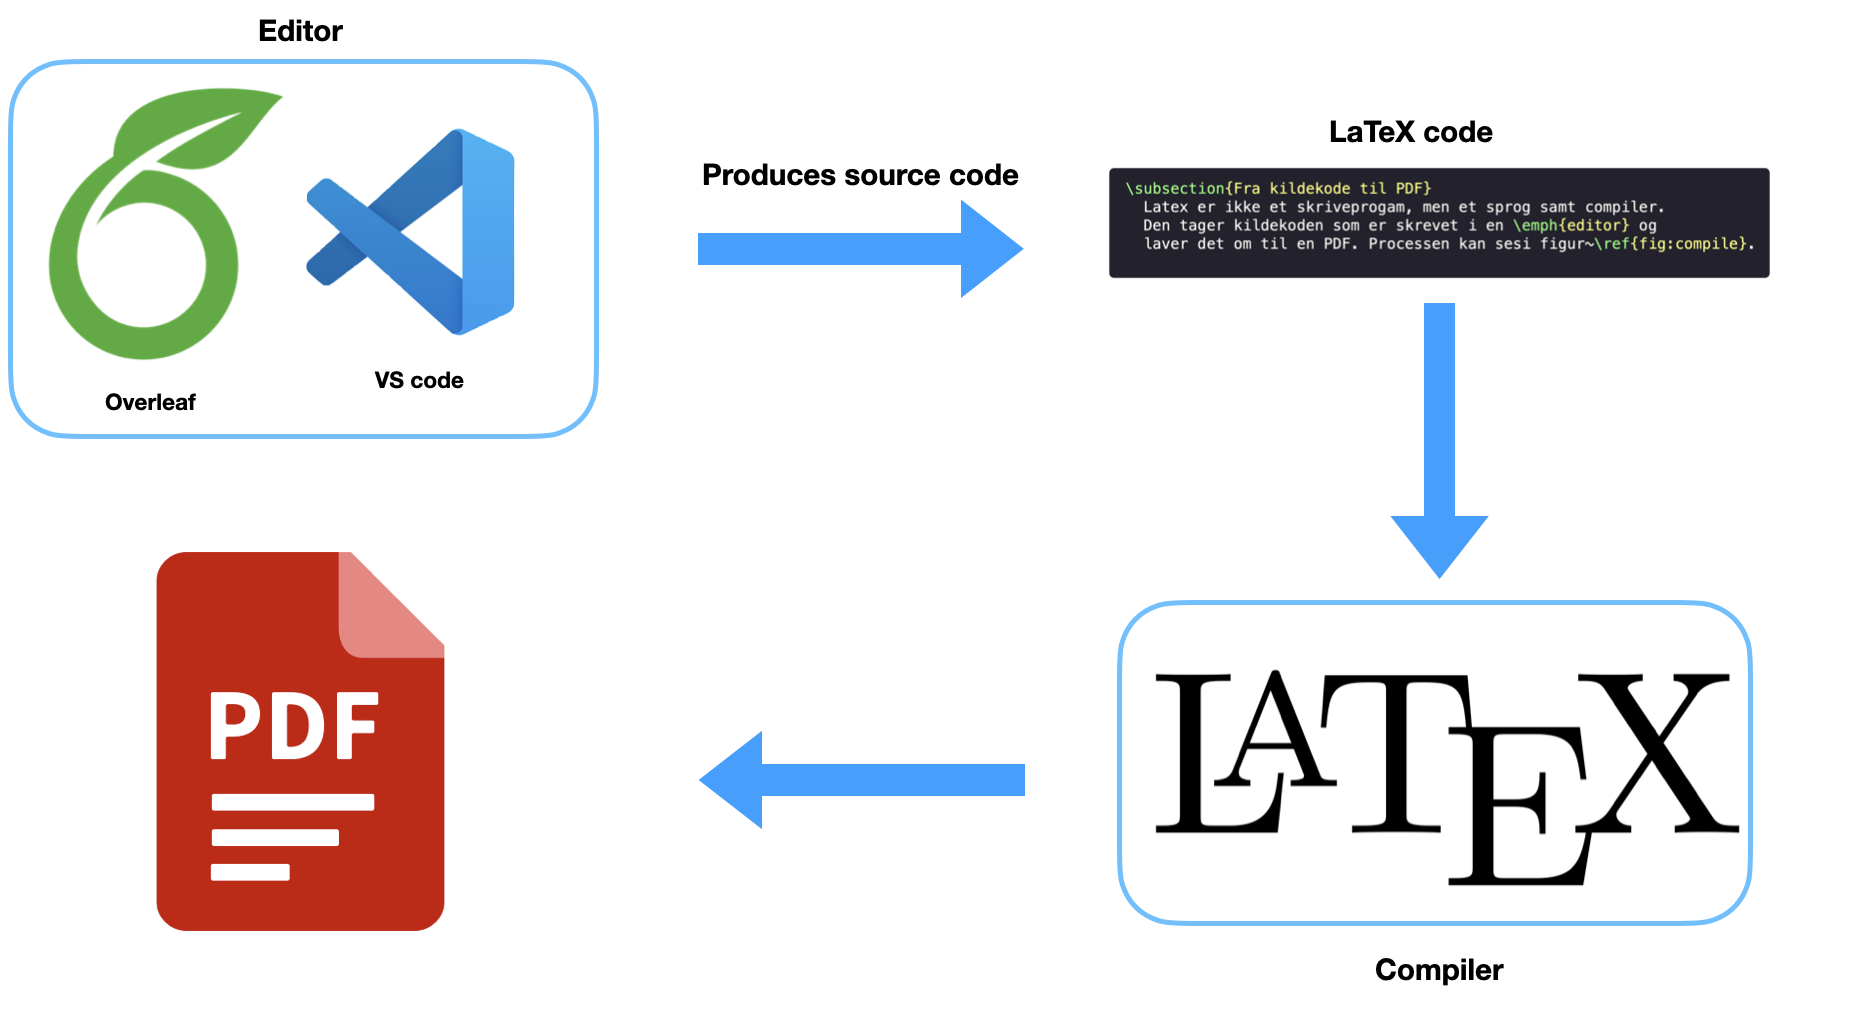
\includegraphics[width=0.9\textwidth]{../assets/compile_en.png}
	\caption{From source code to pdf}\label{fig:compile}
\end{figure}


\section{\LaTeX{} syntax}
In \LaTeX{} we don't click buttons to change formatting, instead we tell the
compiler what type of text we are writing. This leaves the appearance to our
template/compiler leaving us, the writer, to focus on the content.

A \LaTeX{} file consists of two parts, the \emph{preamble} and the document.
The preamble is where we define the \LaTeX{} packages we are going to use,
the style of our document, macros, and other configurations options.
The document is where we write the content.

\subsection{Command syntax}
A command consists of a ``backslash'' followed by a command name. If the
command takes parameters they are written after the command name in curly
parenthesis. As an example if we want to write \LaTeX{} we type \tex{\LaTeX}.
Below is a list of the most common syntax constructs.
\begin{description}
	\item[New lines] \LaTeX{} handles newlines for us, if you write a single
	      line break it will be ignored, so you can format your source code as you
	      wish. If you want to force a line break you can write two line breaks, write
	      \tex{\linebreak} or type two backslashes \tex{\\}.

	\item[Forced spaces] As with line breaks, more than one space are ignored
	      To force a space you can write \tex{\space} or \tex{~~}.

	\item[New page] To force latex to start a new page we type \tex{\newpage}

	\item[Qoutes] To write quotes such as ``Some thing'', we type plings and
	      apostrophes: \tex{``qouted text''}.

	\item[Comments]
	      If you want to type something in your source code but not include it in the
	      final pdf, we can use comments. This is a useful way to leave notes to your
	      future self or group mates. typing \(\%\) will result latex in ignored
	      the remainder of the line. To type  \(\%\), prefix it with a backslash \tex{\%}.


	\item[Math] There are two ways to type math in \LaTeX{}. The first is to
	      \emph{inline}, which places the expression in the flow of the text, i.e \(x^2 +4\),
	      this is done by typing \tex{\(x^2 +4\)}. The other way is \emph{display}
	      mode, where the expression is centered and larger, its written as
	      \tex{\[x^2 +4\]}.  \[x^2 +4\]

	\item[Environemnts]
	      For commands with a large number of parameters we can use the \emph{begin/end}
	      construct. This is done by typing \tex{\begin{environment}[options]\end{environment}}
	      where environment is the name of the environment and options are potential
	      configurations.
\end{description}

Listing~\ref{lst:latex} shows a simple latex-fil, using the above
\LaTeX{} commands.
\begin{listing}[!h]
	\begin{minted}[tabsize=1]{latex}
				\documentclass{article}
				\usepackage{amsmath} % Package for maths
				\usepackage{graphicx} % Package for graphics

				\title{
					\large{Study Now} \\
					\Large{\LaTeX webinar} \\
				}

				\author{
					Benjamin Rotendahl --- Benjamin@Rotendahl.dk
				}

				\begin{document}
						\maketitle
						\section{Introduction}
							This documents gives you \(\dots\)
				\end{document}
   		\end{minted}
	\caption{Example of simple Latex document}\label{lst:latex}
\end{listing}

\subsection{Reference martial and problem solving}
Learning \LaTeX{} is an iterative process, after having learned the basis you
should start using it as much as possible, improving gradually. There are
to many commands to learn all in one sitting. Once you start writing and
run into something you don't know how to do yet, google it and remember it for
next time. For instance if you want to know how to insert two figures side by
side, a google search will most likely lead you to \emph{tex.stackexchange.com}
which has several examples. For more advanced features and a comprehensive
guide, checkout ``The Not So Short Introduction to
\LaTeX\footnote{http://web.math.ku.dk/~holm/download/lshort.pdf}''.


You will often, especially in the beginning, run into errors where the
compiler fails to produce a pdf. The Compiler outputs a log where it tries
to explain what went wrong in a helpful way. As an example if we mistype
and write \tex{\newpge} in stead of \tex{\newpage}, the compiler will write
the following in the log.
\begin{verbatim}[h]
		.../study_now/latex/cheetsheet.tex:241: Undefined control sequence.
		l.241 ...ewpage} we write \newpge
	 \end{verbatim}
The log tells us where the error happened and why. Once you learned to read
the logs you will be able to fix errors quickly.



\section{Math in \LaTeX}
Writing beautifully formatted math is one of the biggest strengths of \LaTeX{}.
We start by telling the compiler to enter \emph{math mode}, it will then parse
the following text as math. It's the difference between y+x and \(y+x\). Many
commands only work in math mode, If you write \tex{\pi} in a non math mode
the compiler will fail. Instead we write \tex{\(\pi\)}, resulting in \(\pi\).

For larger math expressions we can use the \emph{display} mode, which is invoked
by typing \tex{\[x+y\]} or by using the \tex{\equation} environment.
Using the second approach makes it possible to create references to formulas.
As an example the equation \eqref{dot} shows the dot product of two vectors.
\begin{equation}\label{dot}
	\vec{a} \cdot \vec{b} = \sum_{i=1}^{n} a_i b_i
\end{equation}
multiline eqatuon
\begin{flalign*}
	f(x, y)                       & = 3x^2 y + y \\
	\frac{\partial f}{\partial x} & = 6x y       \\
	\frac{\partial f}{\partial y} & = 3x^2  + 1  \\
\end{flalign*}


The code to create the above expression is is shown in listing~\ref{lst:dot}.
\begin{listing}[!h]
	\begin{minted}[tabsize=1]{latex}
		\begin{equation}\label{dot} % Label to reference
			\vec{a} \cdot \vec{b} = \sum_{i=1}^{n} a_i b_i
		\end{equation}
	\end{minted}
	\caption{Equation for the dot product}\label{lst:dot}
\end{listing}

If we wish to have multiple steps in a derivation we can use the \tex{flalign}
environment. This is a way to align equations in a derivation, we type each
line use \tex{\\} to start a new line and set the \tex{&} symbol to specify
the symbol of each line that should be centered.
\begin{flalign}
	f(x, y)                       & = 3x^2y + y^2 \\
	\frac{\partial f}{\partial x} & = 6xy         \\
	\frac{\partial f}{\partial y} & = 3x^2 + 2y
\end{flalign}
The code to produce the above can be seen in ~\ref{lst:diff}. If you don't want
line numbers on the right hand side type \tex{flalign*} instead of \tex{flalign}.
\begin{listing}[!h]
	\begin{minted}[tabsize=1]{latex}
		\begin{flalign}
			f(x, y)                       & = 3x^2y + y^2 \\
			\frac{\partial f}{\partial x} & = 6xy         \\
			\frac{\partial f}{\partial y} & = 3x^2 + 2y
		\end{flalign}
 \end{minted}
	\caption{Example to create multi line math}\label{lst:diff}
\end{listing}
To write parenthesis in formulas we can type them normally, but this will not
scale them according to their contents. To scale them type \tex{\left ( x^2 \right )}
to use different types of parenthesis replace the symbol after \tex{\left, \right}.
Listing~\ref{lst:par} shows the source for the following example
\begin{flalign*}
	f(x) & = (\frac{1}{x})^2                              \\ % Non scaled
	f(x) & = \left ( \frac{1}{x} \right )^2               \\ % Scaled
	x    & \in \left [ \frac{1}{4},  \frac{1}{2} \right ] \\ % Scaled brackets
	x    & \in \left
	\{\frac{1}{n}, \frac{2}{n}, \frac{3}{n}, \dots, \frac{n}{n} \right \}
\end{flalign*}

\[
	\left ( \frac{2}{4} \right )
\]


\subsection{Matrices \& Vectors}
\LaTeX{} makes it easy to write vectors and matrices. It's done by using the
environments: \\\tex{\pmatrix, \bmatrix, \bMatrix} which respectively creates
a matrix with \( (, [, \{ \). In the environemnt you write the rows using
\tex{&} to seperate the elements and \tex{\\} to seprate the rows. The
following example used the code in listing~\ref{lst:matrix}. Note that
the command \tex{\quad} was used to create spacing between the matrices and
that the last matrix used the \tex{\dots, \vdots, \ddots} commands.
\[
	\begin{pmatrix}
		1 & 2 & 3 \\
		4 & 5 & 6 \\
		7 & 8 & 9
	\end{pmatrix}
	,\quad
	\begin{bmatrix}
		1 & 2 & 3 \\
		4 & 5 & 6 \\
		7 & 8 & 9
	\end{bmatrix}
	,\quad
	\begin{Bmatrix}
		1 & 2 & 3 \\
		4 & 5 & 6 \\
		7 & 8 & 9
	\end{Bmatrix}
	,\quad
	\begin{bmatrix}
		1      & \dots  & n      \\
		\vdots & \ddots & \vdots \\
		n      & \dots  & n
	\end{bmatrix}
\]

\[
	\begin{bmatrix}
		1 & 2 & 3 \\
		2 & 3 & 3 \\
		3 & 1 & 2
	\end{bmatrix}
\]


\section{Figures}
To create figures with images and graphs we can use the \tex{figure}
environment. A figure is \emph{floating} element, \LaTeX{} will place the
figure in the document to minimize blank space.
\begin{listing}[!h]
	\begin{minted}[tabsize=1]{latex}
     \begin{figure}[h]
       \centering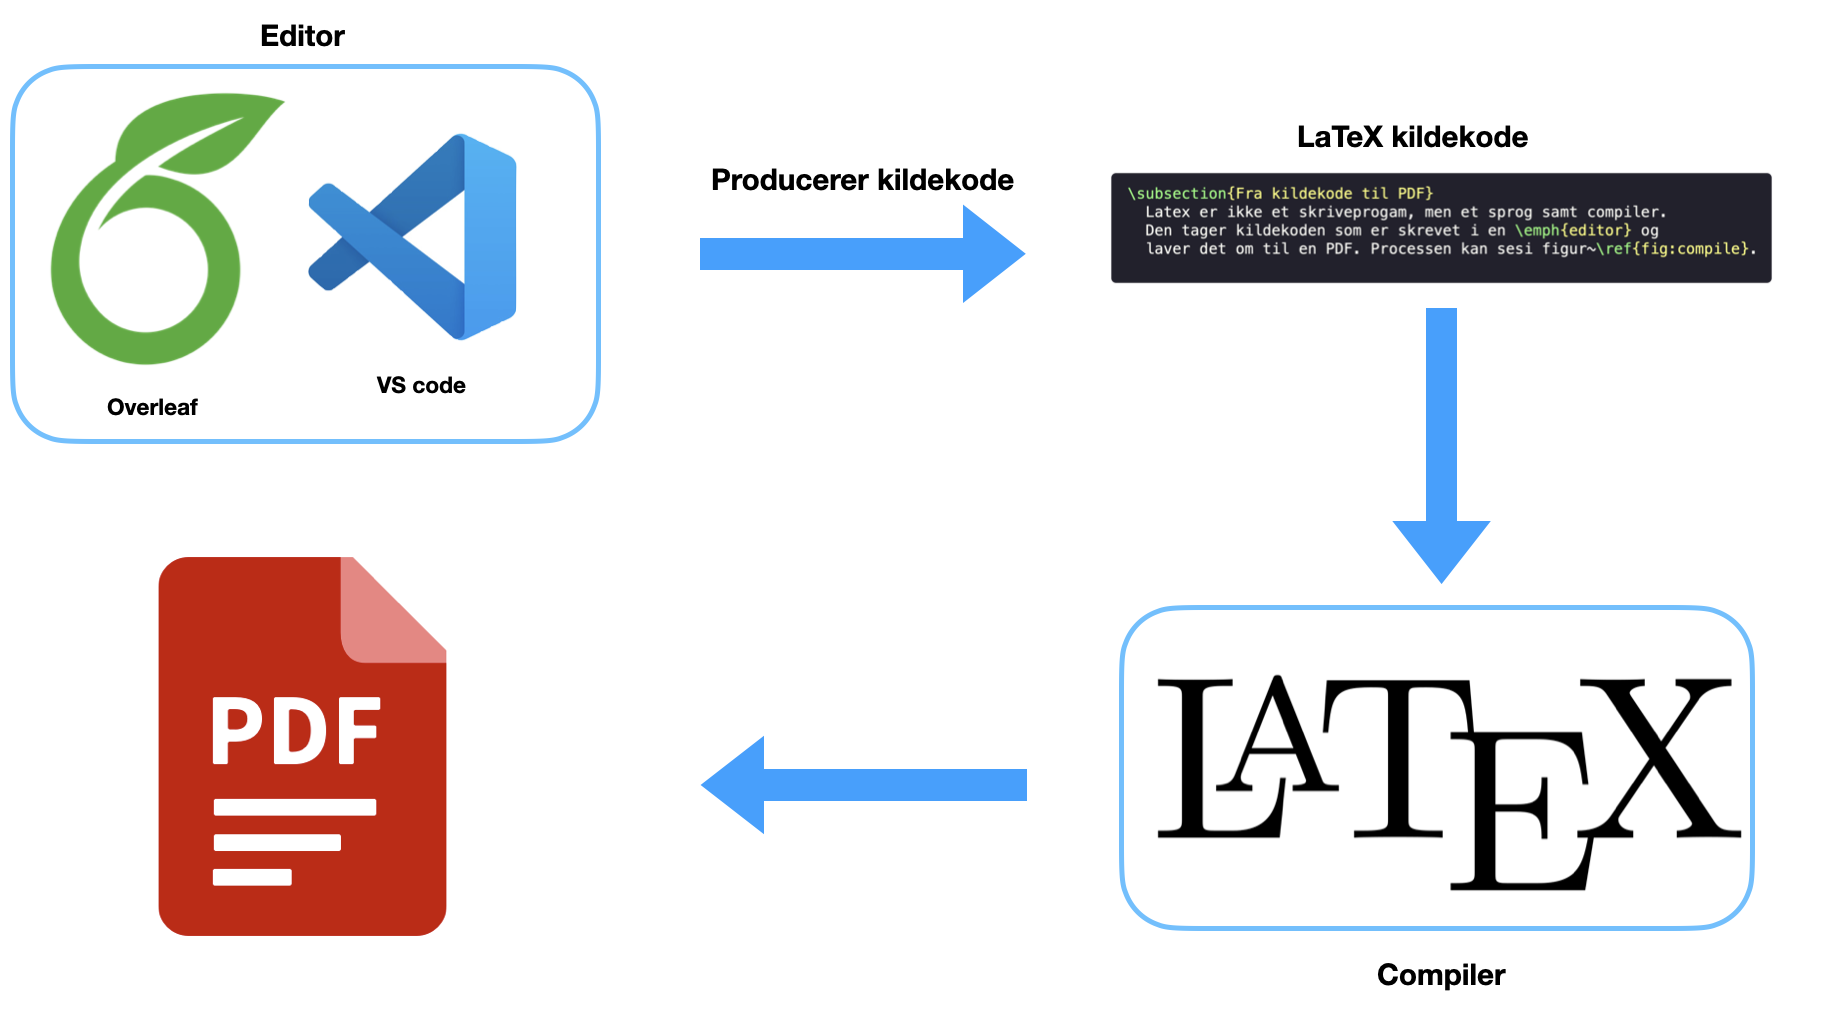
\includegraphics[width=0.9\textwidth]{assets/compile.png}
       \caption{From source coude to pdf}\label{fig:compile}
     \end{figure}
   \end{minted}
	\caption{Example of inserting a figure}\label{lst:figure}
\end{listing}
We create a figure environment, adding the \tex{[h]} option to indicate that
we prioritize having the figure close to the text. \emph{h} could be replaced by
\tex{[t], [b]} which would place the figure at the top or bottom of the page
respectively. The  \tex{\centering} command places the figure in the middle,
and  \tex{\includegraphics} inserts the image, the \tex{\width=.9} specified
the width of the image to \(90\%\) of the page width. The last part of the \tex{\includegraphics}
command in curly parenthesis is the to the file file. Using \tex{\caption} and
\tex{\label} we create a description of the figure and a label to reference.



\subsection{TikZ}
Using the tikz extension we can create our own graphs and figure directly from
latex. TikZ is as powerful as it complex, learning it takes time and effort.
Creating the graphs in another tool and exporting a png is also a viable option.
Figure~\ref{fig:tikz} shows a graph created in TikZ and listing ~\ref{lst:tikz}
shows how it was created.
\begin{figure}
	\centering
	\begin{tikzpicture}
		\begin{axis}[xmax=9,ymax=9, samples=100]
			\addplot[blue, thick] (x,5*x^3+3*x);
			\addplot[red, thin] (x*x,x);
		\end{axis}
	\end{tikzpicture}
	\caption{Example of a tikz graph}\label{fik:tikz}
\end{figure}

\section{Lists}
\begin{description}
	\item[someting:] thing1
	\item[someting:] thing 2
	\item[someting:] sub list  \begin{description}
		      \item[someting:] thing1
		      \item[someting:] thing 2
		      \item[someting:] thing 3
	      \end{description}
\end{description}


\section{Tables}
\begin{table}[h]
	\centering
	\begin{tabular}{l | c  c c}
		\hline
		column1 & column2 & column3 & column4 \\  \hline
		1       & 6       & 87837   & 787     \\
		2       & 7       & 78      & 5415    \\
		3       & 545     & 778     & 7507    \\
		4       & 545     & 18744   & 7560    \\
		5       & 88      & 788     & 6344    \\
		\hline
	\end{tabular}
	\caption{Example of table}\label{table:data}
\end{table}


\begin{table}[h]
	\centering\csvautotabular{../assets/dices.csv}
	\caption{Automatic table from csv}\label{table:dices}
\end{table}


\section{Code listings}
\begin{listing}[!h]
	\begin{lstlisting}[language=python, tabsize=1]
     def fib(x):
       if x == 1 or x == 2:
         return 1
       else:
         return fib(x-1) + fib(x-2)
     \end{lstlisting}
\end{listing}

\section{References}
as shown in\cite{attention}


\newpage
\appendix
\bibliography{../assets/references}{}
\bibliographystyle{plain}


\end{document}
